% TODO: Template out all the things that change document to document
%             and put them in the default.properties file

% Stuff that may change from year to year; also check slide s:other-courses
%\newcommand{\coursepath}{/teaching/2425/ConcDisSys/}
\newcommand{\courseurl}{\url{$course_url$}}
\newcommand{\thisyear}{$this_year$}

\newcommand{\mydetails}{%
    $instructor_name$ \\\\
   $instructor_email$  \\\\[1em]
   $organization$  \\\\
}

\fancypagestyle{plain}{%
  \renewcommand{\headrulewidth}{0pt}%
  \fancyhf{}%
  \fancyfoot[C]{%
    % \raisebox{-0.15cm}{
\includegraphics[height=0.5cm]{images/creative-commons.png}}\hspace{5pt}
    \raisebox{-0.15cm}{\colorbox{gray}{\rule{0.5cm}{0.5cm}}}\hspace{5pt}
      This work is published under a \href{https://creativecommons.org/licenses/by-sa/4.0/}{Creative Commons BY-SA license}.%
  }%
}

\begin{document}
\title{ $title$ }
\subtitle{ $organization$ \\\\%
$course_term$ \thisyear\\\\%
\courseurl}

\author{ $instructor_email$ \\\\ $instructor_email$ }
\date{}
\maketitle
\tableofcontents

\vspace{10pt}\noindent Thank you (TODO acknowledgements).

\def\sectionautorefname{Section}%
\def\subsectionautorefname{Section}%
\def\subsubsectionautorefname{Section}%

% Include all bib file entries in document even if they're not
% explicitly cited.  Remove this line once you actually start citing
% things if you don't want unreferenced bibliographic items to
% appear.  Keep this line if you want to build to not break before any
% citations are made.
\nocite{*}

\newpage
\section{Introduction}\label{sec:introduction}

%%%%%%%%%%%%%%%%%%%%%%%%%%%%%%%%%%%%%%%%%%%%%%%%%%
% TODO: Add some example slides the demonstrate useful things
%%%%%%%%%%%%%%%%%%%%%%%%%%%%%%%%%%%%%%%%%%%%%%%%%%

\lipsum[1]

% EXAMPLE: Slide with some TikZ graphics in it
\begin{frame}
    \label{s:shared-memory}
    \frametitle{Two models of concurrency}
    Shared-memory concurrency:
    \begin{center}
        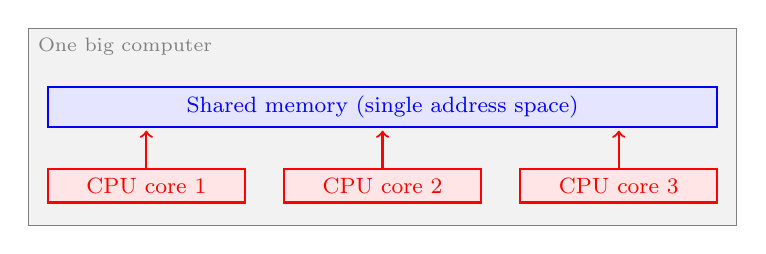
\begin{tikzpicture}
            \tikzstyle{cpu}=[draw=red, fill=red!10, thick, minimum width=2.5cm, font=\footnotesize]
            \tikzstyle{memory}=[blue, draw=blue, fill=blue!10, thick, minimum width=8.5cm, font=\footnotesize]
            \draw [black!50, fill=black!5] (0, 0) rectangle (9, 2.5);
            \node [black!50, anchor=north west, font=\scriptsize] at (0, 2.5) {One big computer};
            \node [memory] at (4.5, 1.5) {Shared memory (single address space)};
            \draw [thick, red, ->] (1.5, 0.5) node [cpu] {CPU core 1} -- (1.5, 1.2);
            \draw [thick, red, ->] (4.5, 0.5) node [cpu] {CPU core 2} -- (4.5, 1.2);
            \draw [thick, red, ->] (7.5, 0.5) node [cpu] {CPU core 3} -- (7.5, 1.2);
        \end{tikzpicture}
    \end{center}

    Message-passing distributed systems:
    \begin{center}
        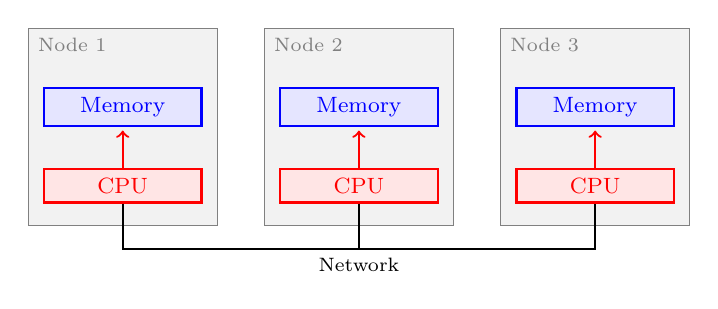
\begin{tikzpicture}
            \tikzstyle{machine}=[black!50, anchor=north west, font=\scriptsize]
            \tikzstyle{cpu}=[draw=red, fill=red!10, font=\footnotesize, thick, minimum width=2cm]
            \tikzstyle{memory}=[blue, draw=blue, fill=blue!10, font=\footnotesize, thick, minimum width=2cm]
            \draw [machine, fill=black!5] (0.3, 0) rectangle (2.7, 2.5);
            \draw [machine, fill=black!5] (3.3, 0) rectangle (5.7, 2.5);
            \draw [machine, fill=black!5] (6.3, 0) rectangle (8.7, 2.5);
            \node [machine] at (0.3, 2.5) {Node 1};
            \node [machine] at (3.3, 2.5) {Node 2};
            \node [machine] at (6.3, 2.5) {Node 3};
            \node [memory] at (1.5, 1.5) {Memory};
            \node [memory] at (4.5, 1.5) {Memory};
            \node [memory] at (7.5, 1.5) {Memory};
            \draw [thick, red, ->] (1.5, 0.5) node [cpu] (t1) {CPU} -- (1.5, 1.2);
            \draw [thick, red, ->] (4.5, 0.5) node [cpu] (t2) {CPU} -- (4.5, 1.2);
            \draw [thick, red, ->] (7.5, 0.5) node [cpu] (t3) {CPU} -- (7.5, 1.2);
            \draw [thick] (t1.south) -- (1.5, -0.3) -- (7.5, -0.3) -- (t3.south);
            \draw [thick] (t2.south) -- (4.5, -0.3);
            \node [anchor=north, font=\scriptsize] at (4.5, -0.3) {Network};
        \end{tikzpicture}
    \end{center}
\end{frame}
\inlineslide{s:shared-memory}{}



\footnotesize
\bibliographystyle{plainnat}
\bibliography{references}{}
\end{document}
